\label{analysis-results}
\chapter{Initial Results} 

\begin{abstract}
This chapter will present individual results of each of the model+method pairings without any direct comparisons made. Each pairing combines one model variation with one decision support method, both based on the configurations developed in \cref{part-develop}. The individual results provide a foundation for the comparisons made next, in \cref{chapter-comparison}. Results will be presented in three stages: policy alternative determination in \cref{results-step2}, uncertainty analysis in \cref{results-step3}, and finally scenario discovery in \cref{results-step4}. As the model specification phase does not include any direct results apart from the development of models that are used in the remaining steps, and as the model variations do not change based on the method used, there is no specific section that covers that step in this chapter. For details on the implementation of each model variation, see \cref{dev-step1}. 
\end{abstract}

\newpage

\section{Step 2: Policy Alternative Determination} \label{results-step2}
Given a model, the next step of the analysis for each of the three methods under consideration is to search for a set of non-dominated policy alternatives. This section examines the outcome of that search, including convergence behavior and the resulting set of non-dominated alternatives. 

    \subsection{Convergence of the search process} \label{results-convergence}
    The search process used in this analysis included several convergence metrics, which are used to track the progress and stabilization of the search process. This section will discuss the results of two of the most commonly used metrics: epsilon progress and hypervolume convergence \citep{Reed2013,Ward2015}. Epsilon progress indicates whether new policies are being added to the set of non-dominated alternatives as the search progresses \citep{Ward2015}. Of interest for this metric is the slope of the epsilon progress line. A flat slope means that few or no new policies are being added to the set of non-dominated alternatives, indicating that the search process is no longer finding new alternatives. The goal of an MOEA-based search in the context of epsilon progress is to use enough functional executions to reach the point when the slope flattens out.
    
    Hypervolume provides a picture of the possible objective space that is being covered by a set of policy alternatives, given the boundaries of the space that is provided to the search algorithm \citep{Reed2013}.  See \cref{table:moeaadditional} for the hypervolume settings used in this analysis. Again, of interest is the slope of hypervolume curves. A flatter slope indicates that, even if new policies are being added to the set of non-dominated alternatives, those policies are not contributing to the diversity of the set of non-dominated alternatives. Therefore, those new additions do not reveal any significantly new information about potentially successful combinations of decision lever settings.
    
    Both of these metrics are plotted for every model+method pairing. Given that multiple independent repetitions were performed for each model+method search in order to reduce the impact of randomness that exists in the MOEA, one curve in a plot corresponds to one search repetition. In addition to the two plots that show the epsilon progress and hypervolume as the number of function executions builds, there is a plot of the relationship between hypervolume and epsilon progress. Of interest here is a positive correlation between hypervolume and epsilon progress, indicating that as the search adds new alternatives to the non-dominated set, it also increases the diversity of that set. A flat, horizontal slope here indicates that even though new alternatives are being added to the set of non-dominated policies, those new alternatives are not contributing to the diversity of the set. This is another indication of the stabilization of the search process. For a discussion of the other convergence metrics that were configured, which track the use of each of the five operators in the auto-adaptive NSGAII algorithm, see \cref{appendix-operatorconvergence}.
    
    As a note, the convergence metrics for all five reference scenarios of multi-scenario MORDM are plotted on the same chart. The reference scenarios each display different convergence trends. For example, the hypervolume and maximum epsilon progress of the non-dominated sets of policy alternatives found using each reference scenario converge to different values. The difference in values with respect to stabilization is important to keep in mind as the convergence plots for multi-scenario MORDM are presented.
    
        \subsubsection{Intertemporal}
        Due to computational and memory constraints, the number of functional executions for the intertemporal lake model changes per method. For both MORDM and multi-scenario MORDM, 500,000 functional executions are used. For the MORO method, 300,000 functional executions are used. \cref{fig:convergences-inter-planned} contains the convergence visualization for each method.
        
        In general, these plots show that the MOEA search is able to reach a stable epsilon progress and hypervolume, with quite consistent results for MORDM-based analysis. The MORO convergence plots do indicate a fairly significant early difference in the hypervolume, but that this value trends toward a much more similar final hypervolume (save one exception).

        \begin{figure}[H]
            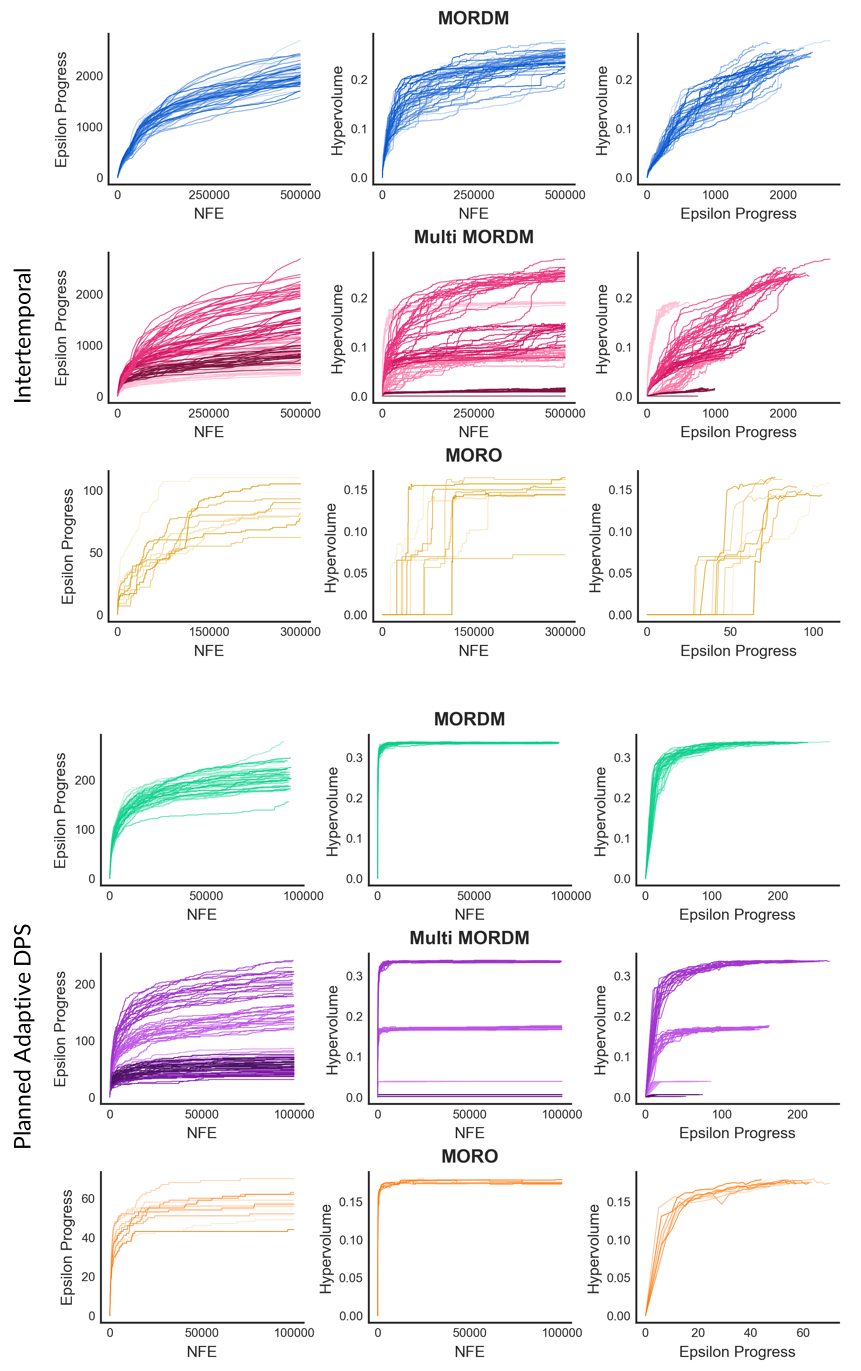
\includegraphics[height=\dimexpr
            \textheight-2\baselineskip-\abovecaptionskip-\belowcaptionskip\relax]{convergences/convergences_inter_planned}
            \caption[Convergences for the intertemporal and planned adaptive DPS variations]{Intertemporal and Planned Adaptive DPS convergences for each method. The first two plots in each row show the the relationships between epsilon progress, hypervolume, and number of function executions (NFE). The third shows the relationship between hypervolume and epsilon progress.}
            \label{fig:convergences-inter-planned}
        \end{figure}
        
        \begin{figure}[H]
            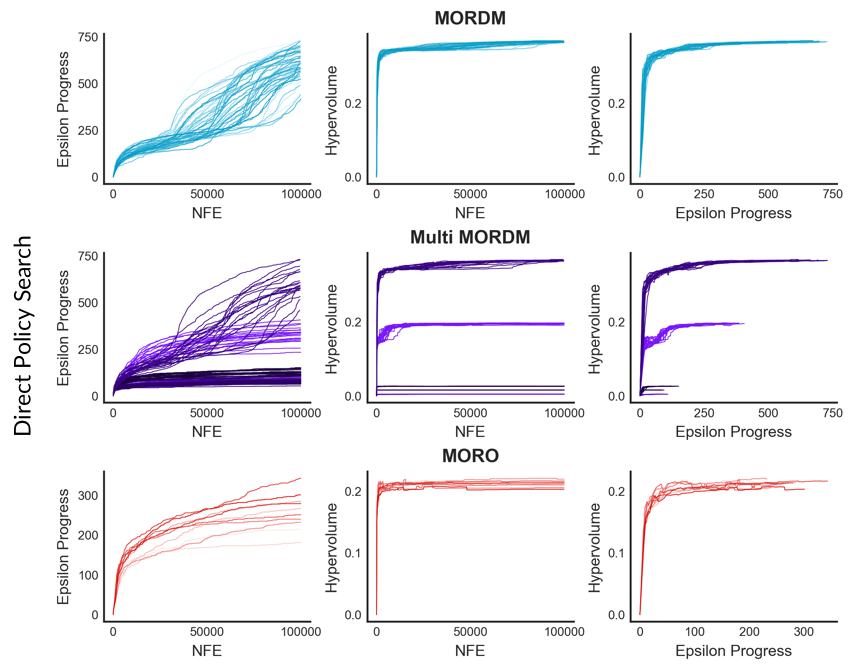
\includegraphics[width=\textwidth]{convergences/convergences_dps}
            \caption[Convergences for the DPS variation]{DPS convergences for each method. The first two plots in each row show the the relationships between epsilon progress, hypervolume, and NFE. The third shows the relationship between hypervolume and epsilon progress.}
            \label{fig:convergences-dps}
        \end{figure}

        As noted, the multi-scenario MORDM convergences for the intertemporal problem variation include convergences to different maximum epsilon progress values and hypervolumes. Despite the differences in maximum values seen between the different reference scenarios, each scenario independently reaches stabilization. 

        \subsubsection{Planned adaptive DPS}
        The planned adaptive lake problem used 100,000 function executions in each method's search phase to build non-dominated sets of policy alternatives. The search processes built convergences that are plotted in \cref{fig:convergences-inter-planned}, where each curve represents one repetition of the search process. 
        
        Across all methods, these plots indicate rapid and fairly consistent convergence to a stable hypervolume. Additionally and similar to the intertemporal problem, each reference scenario in multi-scenario MORDM analysis yield different but rapidly converging hypervolumes. Epsilon progress also levels off quite quickly for all methods, and there is a consistent and stable correlation between hypervolume and epsilon progress. All of these pieces of information, together, indicate a consistently successful search process, in terms of convergence. Furthermore, similar behavior is seen for the multi-scenario MORDM method in the case of planned adaptive DPS as was described for the intertemporal problem variation. Though each reference scenario stabilizes at a different value for hypervolume and epsilon progress, stabilization still occurs at a similar rate and by the final function execution of the search process. 

        \subsubsection{DPS}
        The DPS lake problem also used 100,000 function executions in each method's search process to build non-dominated sets of policy alternatives. The search processes built convergences that are plotted in \cref{fig:convergences-dps}, where each curve represents one repetition of the search process. 
        
        The hypervolume values of each method converge quite quickly to a small range of values. Epsilon progress also flattened out as the search process continued in the MORO and for most reference scenarios in the multi-scenario MORDM methods. The MORDM search process, using the base reference scenario specified in \cref{table:uncertainties} and which corresponds to the reference scenario in the multi-scenario MORDM plots with similar behavior, indicates both flat stretches and significant increases in epsilon progress throughout the search process, depending on the repetition. However, when the hypervolume convergence and relationship between epsilon progress and hypervolume are considered along with isolated epsilon progress, the changes in epsilon progress do not seem to add diversity to the non-dominated set of policy alternatives after the very early stages of search. This indicates that an NFE of 100,000 is sufficient to determine as diverse a set of non-dominated policy alternatives as possible. 
        
        Finally and similar to the intertemporal and planned adaptive DPS variations, the plots for multi-scenario MORDM for the DPS variation indicate that each reference scenario converges to a different hypervolume and epsilon progress. However, each reference scenario is still able to reach stabilization. 
        
    \begin{table}[ht]
        \centering
        \caption[Size of non-dominated policy alternative sets]{Size of the final non-dominated set of policy alternatives for each method and variation of the lake problem}
        \label{table:paretosize}
        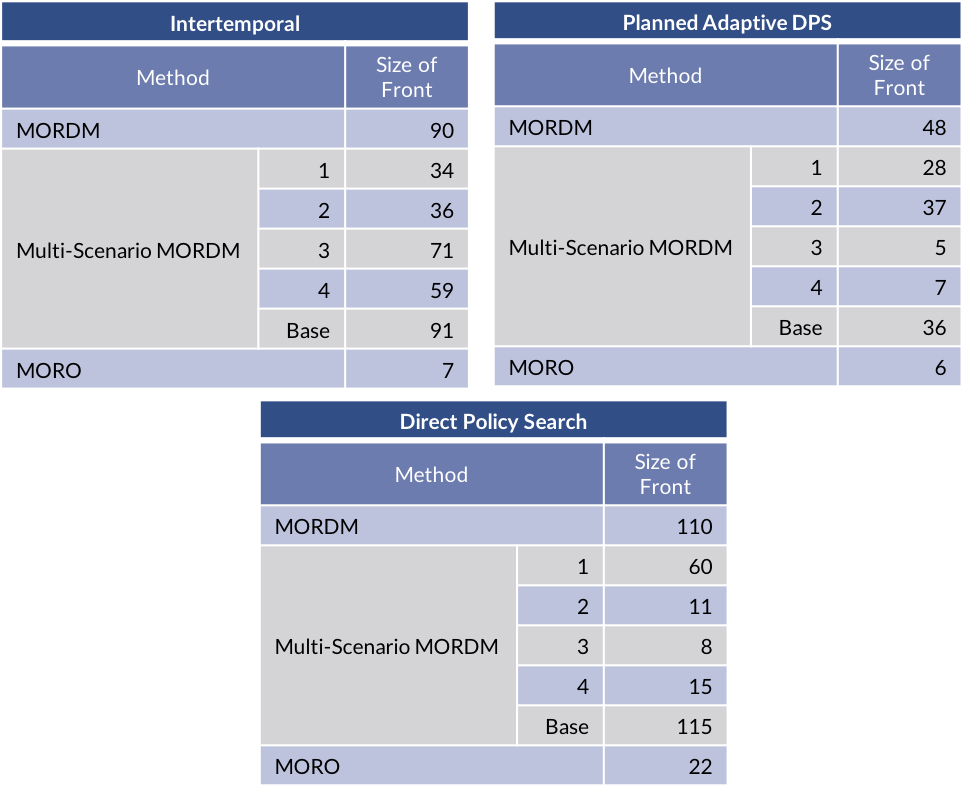
\includegraphics[width=\textwidth]{convergences/pareto_front}
    \end{table}
    
    \begin{figure}[ht]
        \centering
        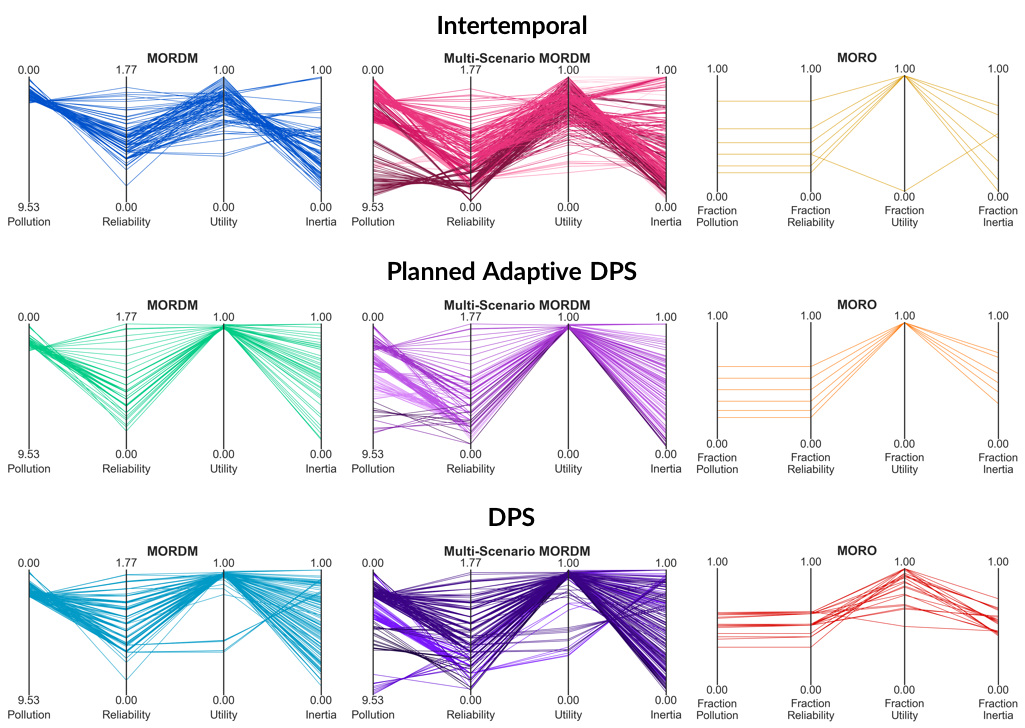
\includegraphics[width=\textwidth]{convergences/nondominated_outcomes_all}
        \caption[Outcome value ranges across all pairings]{Ranges of outcome values for each member of the non-dominated set of policy alternatives. The desirable values for each outcome are at the top. The outcomes of interest for MORDM and multi-scenario MORDM analysis are absolute values that indicate the performance of that policy given the reference scenario. The outcomes of interest for MORO-based analyses is based on robustness, where a single value is the fraction of cases that meet the identified threshold from the set of scenarios used in a MORO-based search.}
        \label{fig:nondominated-outcomes}
    \end{figure}

    \subsection{Final non-dominated front}
    The non-dominated sets of alternatives generated for each search repetition are a final time to determine the super-set of alternatives that will be considered. The sizes of each final set of policy alternatives are indicated in \cref{table:paretosize}, and the ranges of outcome values that identified each policy are found in \cref{fig:nondominated-outcomes}. 
    
    There are a few key features of these results to point out, listed below. However, for a deeper exploration of the impact of the random seed on the discovered set of policy alternatives, see \cref{appendix-seedanalysis}. 
    
    \begin{itemize}
        \item For all model types, multi-scenario MORDM results produce scenarios over a broader range of maximum pollution levels than the other two methods. 
        \item Planned adaptive DPS and DPS lake models include non-dominated policy alternatives that seem to perform much better at inertia than the intertemporal model. 
        \item MORO results in a significantly smaller number of policy alternatives than the other two methods for all variations of the lake problem. 
    \end{itemize}

\section{Step 3: Uncertainty Analysis} \label{results-step3}
The third phase of analysis for each of the methods under consideration is to explore how each policy reacts to a variety of potential future states of the world through uncertainty analysis. As indicated in the methodology from \cref{dev-step3}, the uncertainty analysis stage is divided into two parts, the first of which is computational exploration. An in depth review of the results of this part can be found in \cref{appendix-uncertainty}. After building an library of experiments and their corresponding outcomes, which indicate each policy alternative's behavior across an ensemble of 10,000 uncertainty settings, policy robustness can be calculated according to the metrics that have been selected. This is the second part of uncertainty analysis. 

In this case, robustness is implemented using Starr's domain criterion measure \citep{Starr1963}. The domain criterion measure is defined as the fraction of experiments that lead to an value that exceeds a specified threshold for an outcome of interest. Specific definitions of robustness for each outcome of interest and their thresholds of acceptability are found in \cref{step0-robust}. The parallel plots in \cref{fig:robust-parallel-all} summarize the robustness of each set of non-dominated policy alternatives, where a robustness value of 1 (at the top of each axis) indicates perfect robustness, while a robustness value of 0 (at the bottom of each axis) indicates a complete failure to meet the threshold for all uncertainty vectors in the ensemble of possible SOWs constructed during computational exploration. 

\begin{figure}[ht]
    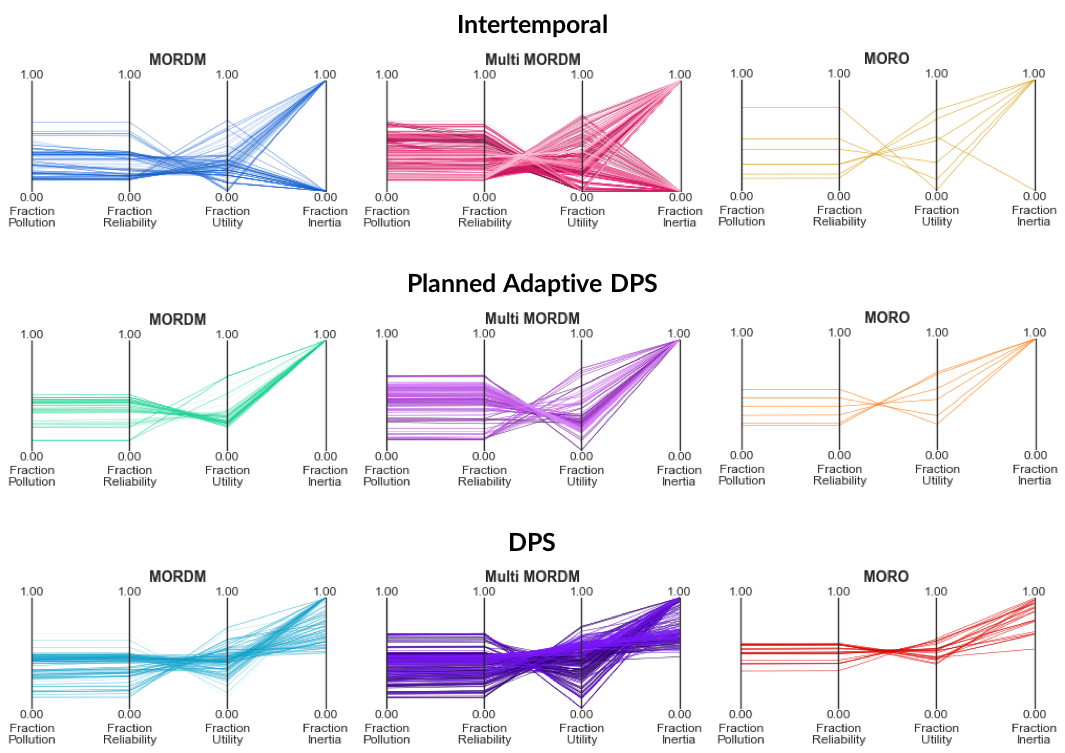
\includegraphics[width=\textwidth]{uncertainty/robust_parallel_all}
    \caption[Robustness value ranges across all pairings.]{Robustness values for policy alternatives across all model and method pairings. Robustness is determined using Starr's domain criterion \citep{Starr1963}. The desirable robustness value is at the top of each axis.}
    \label{fig:robust-parallel-all}
\end{figure}

These plots reveal that all policy alternatives for the planned adaptive DPS lake problem have high levels of inertia-based robustness. They also indicate the primary conflict between the selected outcomes of interest: there is a distinct crossing point between the reliability and utility axes for most, if not all policy alternatives across the board. This would indicate that those two outcomes of interest are generally in conflict with each other. The parallel plot can also reveal outcomes of interest that support one-another through horizontal curves that connect two axes. This is the case with the pollution and reliability outcomes of interest. Both of these trends follow the definitions of each outcome. Both the pollution and reliability metrics reflect on a desire to maintain low or manageable levels of pollution in the lake. And given that utility reflects the desire for industry and agriculture to release pollution into the lake in order to increase their profits, a conflict with the reliability and pollution metrics is expected. 

\begin{figure}[ht]
    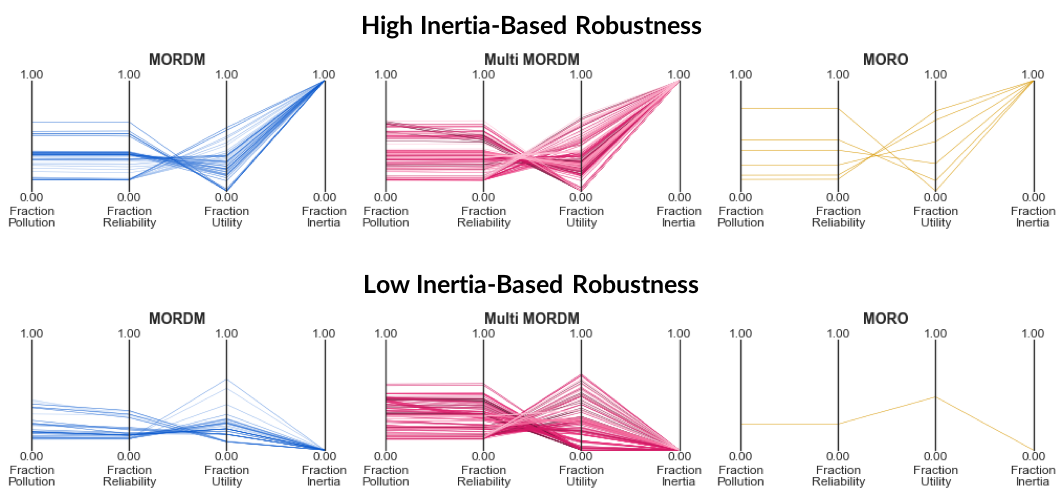
\includegraphics[width=\textwidth]{uncertainty/robust_parallel_moro_inertia}
    \caption{Robust outcome values for the intertemporal lake problem, isolating high and low inertia values.}
    \label{fig:robust-parallel-moro-inertia}
\end{figure}

Interestingly, the non-dominated policy alternatives selected for the intertemporal lake problem result in a wide range of robustness results for inertia that is not seen in the DPS and planned adaptive DPS lake models. Furthermore, the two extremes of inertia seem to be paired with utility robustness values that span the entire active value range. Separating policies that lead to high and low inertia, seen in \cref{fig:robust-parallel-moro-inertia}, does not lead to an obvious trend in robustness values that may indicate common behavior that leads to inertia that is consistently above or below the defined threshold. This type of discovery is what the next step, scenario discovery, is meant to explore and, hopefully, explain.

%TODO EEB scenario discovery on this property in an effort to determine why that happens. 

\section{Step 4: Scenario Discovery} \label{results-step4}
The final component of an RDM analysis as defined by this study is scenario discovery, which involves using PRIM to discover lingering vulnerabilities in the model after the initial search for theoretically robust alternatives. Unlike traditional RDM, which uses the information learned about lingering vulnerabilities to readjust the set of policy alternatives under consideration, these robust decision support methods must return to the model specification step to adjust decision levers or other model characteristics. Only then will the MOEA be able to determine new policy alternatives that may address the vulnerabilities identified. 

Once uncertainty analysis has been completed, the data set generated can be used for scenario discovery. Because this study uses PRIM, the first configuration step involves determining which entries in the data set are of interest. The threshold values of robustness are used here, where an entry is considered of interest if the outcome under consideration falls below its robustness threshold. The scenario discovery process will examine uncertainties in isolation, to determine what ranges of uncertainties may contribute to failure, independent of the policy in effect. Also under consideration is the potential effect of both uncertainties and lever values together, which provides an indication of a common lever and uncertainty pairing that leads to vulnerabilities in the system under consideration. Because the intertemporal variation involves so many decision levers, the policy name is used instead of the set of decision levers to simplify PRIM's search process and to provide a more straightforward way to communicate whether or not a policy impacts the system's vulnerabilities. 

The scenario discovery results for every method and lake problem pairing have indicated that there is no simple rule that explains failure in utility or inertia, given the classification settings used. Each MORDM-based study found that undesirable reliability and pollution outcomes are caused by a range of values for the pollution rate of removal, $b$. \cref{fig:mordm-PRIM} indicates the box limits and quasi-p value (in parenthesis next to the parameter name) for each application of the MORDM method that supports this conclusion. The scenario discovery results for multi-scenario MORDM based analysis and MORO based analysis reach similar conclusions, but with slight variations in the range of values for $b$ that are considered explanatory. 

\begin{figure}[ht]
    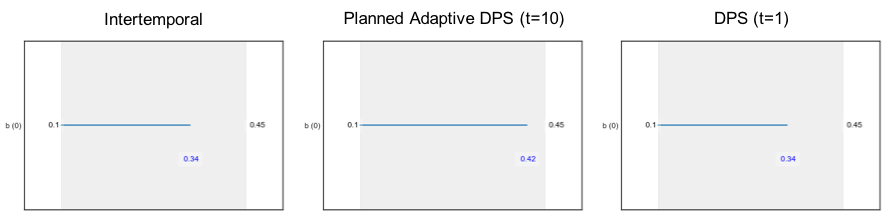
\includegraphics[width=\textwidth]{scenariodiscovery/allmordm_inspect}
    \caption[Results of PRIM Analysis]{Results of the PRIM analysis of the MORDM method applied to each variation of the lake problem. Each figure indicates the box limits when attempting to explain failures of the combined set of outcomes. Failure is indicated when an experiment does not produce an outcome of interest above the robustness threshold defined in \cref{step0-robust}.} 
    \label{fig:mordm-PRIM}
\end{figure}

This scenario discovery process can be enhanced by considering varying thresholds for each outcome of interest, to determine potential causes for different levels of failure. For example, despite not finding any explanatory behavior that caused failure in utility or inertia when classification uses the original robustness threshold, there may be ranges of uncertainties or decision levers that explain failure when robustness does not meet a lower standard (i.e. there are fewer failures to meet the desired utility or inertia setting). By selecting a smaller group of experiments that are of interest, PRIM may prove more effective, as it has been known to struggle with larger sets of experiments that are of interest \citep{Kwakkel2017}. 